\documentclass[aps,pra,10pt,twocolumn,groupedaddress,nofootinbib]{revtex4-1}

\usepackage{amsmath, amssymb, amsthm}
\usepackage{graphicx}% Include figure files
\usepackage{bm,bbm}% bold math
\usepackage{hyperref}% add hypertext capabilities
\usepackage[margin=2cm]{geometry}
\usepackage{xcolor}
\usepackage{algorithm}
\usepackage[noend]{algpseudocode}


\theoremstyle{plain}
\newtheorem{theorem}{Theorem}%[section]


\DeclareMathOperator{\re}{Re}
\DeclareMathOperator{\im}{Im}
\DeclareMathOperator{\tr}{Tr}
\DeclareMathOperator{\Ad}{Ad}
\DeclareMathOperator{\ad}{ad}
\DeclareMathOperator{\diag}{diag}  % diagonal vector of the given matrix / diagonal matrix with the given vector as diagonal
\DeclareMathOperator{\Ker}{Ker}    % kernel
\DeclareMathOperator{\Imag}{Imag}  % image
\DeclareMathOperator{\spec}{spec}  % eigenvalue spectrum
\DeclareMathOperator{\lcm}{lcm}    % least common multiple

\newcommand{\isom}{\cong} % isomorphic to
\newcommand{\conj}[1]{\overline{#1}} % complex conjugate
\newcommand{\mnorm}[1]{\ensuremath{\left\| #1 \right\|}} % matrix norm

\newcommand{\de}[2]{\frac{d #1}{d #2}}   % derivative
\newcommand{\pd}[2]{\frac{\partial #1}{\partial #2}}  % partial derivative
\newcommand{\hc}{\text{h.c.}}  % hermitian conjugate

\newcommand{\be}{\begin{equation}}
\newcommand{\ee}{\end{equation}}
\newcommand{\bpm}{\begin{pmatrix}}
\newcommand{\epm}{\end{pmatrix}}

\newcommand{\naturals}{\ensuremath{\mathbb N}}
\newcommand{\Z}{\ensuremath{\mathbb Z}}  % integer numbers
\newcommand{\Q}{\ensuremath{\mathbb Q}}  % rational numbers
\newcommand{\R}{\ensuremath{\mathbb R}}  % real numbers
\newcommand{\C}{\ensuremath{\mathbb C}}  % complex numbers
\newcommand{\K}{\ensuremath{\mathbb K}}  % any field
\newcommand{\I}{\mathbbm{1}} % vector space identity op

\newcommand{\SL}{\text{SL}} % special linear group
\newcommand{\GL}{\text{GL}} % general linear group
\newcommand{\OO}{\text{O}}  % orthogonal group
\newcommand{\SO}{\text{SO}} % special orthogonal group
\newcommand{\U}{\text{U}}   % unitary group
\newcommand{\SU}{\text{SU}} % special unitary group
\newcommand{\Sp}{\text{Sp}} % symplectic group


\newcommand{\CNOT}{\text{CNOT}}

\newcommand{\comm}[2]{\ensuremath{\left[#1, #2\right]}}             % commutator
\newcommand{\acomm}[2]{\ensuremath{\left\{#1, #2\right\}}}          % anticommutator
\newcommand{\ket}[1]{\ensuremath{\left| #1 \right \rangle}}
\newcommand{\bra}[1]{\ensuremath{\left \langle #1 \right |}}
\newcommand{\braket}[2]{\ensuremath{\left\langle #1\left|#2 \right.\right\rangle}}
\newcommand{\ketbra}[2]{\ket{#1}\bra{#2}}
%\newcommand{\vect}[1]{\ensuremath{\mathbf{#1}}}
\newcommand{\inprod}[2]{\ensuremath{\left\langle #1, #2 \right\rangle}}  % inner product
\newcommand{\lieprod}[2]{\ensuremath{\left[#1, #2\right]}}          % Lie product
\newcommand{\liealg}[1]{\ensuremath{\mathfrak{#1}}}                 % Lie algebra
\newcommand{\expect}[1]{\ensuremath{\left\langle #1 \right\rangle}} % expectation value
\newcommand{\tracep}[1]{\ensuremath{\trace\left( #1 \right)}}


\renewcommand{\a}{\hat{a}}
\newcommand{\adag}{\hat{a}^{\dagger}}
\newcommand{\x}{\hat{x}}
\newcommand{\p}{\hat{p}}
\newcommand{\bx}{\mathbf{x}}
\newcommand{\bp}{\mathbf{p}}
\newcommand{\bq}{\mathbf{q}}
\newcommand{\e}{\mathrm{e}}
\newcommand{\bad}{\bm{\hat a}^\dagger}
\renewcommand{\L}{\mathcal{L}}
\newcommand{\G}{\mathcal{G}}

\newcommand{\sidenote}[1]{\marginpar{\footnotesize{\textcolor{red}{-#1}}}}

\newcommand{\nathan}[1]{\textcolor{blue}{Nathan: #1}}
\newcommand{\maria}[1]{\textcolor{orange}{Maria: #1}}
\newcommand{\ville}[1]{\textcolor{purple}{Ville: #1}}

%quantum and classical node stypes
\usepackage{tikz}
\usetikzlibrary{calc}
\usetikzlibrary{shapes.multipart}
\definecolor{quantum1}{HTML}{8EDBCE}
\definecolor{quantum2}{HTML}{3F605B}
\definecolor{exp1}{HTML}{9AB9ED}
\definecolor{exp2}{HTML}{204177}
\definecolor{classical}{HTML}{EBBA92}
\tikzset{input node/.style={}}
\tikzset{quantum node/.style={draw, align=center, anchor=west, inner sep=5pt,rounded corners=4pt, rectangle split, rectangle split horizontal, rectangle split parts=2, rectangle split part fill={quantum1,quantum2}, every two node part/.style={text = white}}}
\tikzset{classical node/.style={draw, rectangle,align=center, anchor=west, thin, fill=classical, inner sep=5pt}}
%\tikzset{expectation node/.style={draw, align=center, anchor=west, inner sep=5pt, rectangle split, rectangle split horizontal, rectangle split parts=2, rectangle split part fill={exp1,exp2}, every two node part/.style={text = white}}}
\tikzset{output node/.style={}}
\tikzset{out label/.style={midway, above}}
\tikzset{connector/.style={anchor=center, opacity=0.}}
\tikzset{samples label/.style={at start, below, xshift=4pt}}


\begin{document}

\title{OpenQML - Technical manuscript}
\author{Maria Schuld}
\author{Nathan Killoran}
\email{nathan@xanadu.ai}
\author{Ville Bergholm}
\affiliation{Xanadu Inc., 372 Richmond St W, Toronto, M5V 1X6, Canada}


\date{\today}

\begin{abstract}
Compilation of formulas and conventions for the OpenQML framework.
\end{abstract}

\maketitle


\section{Conventions}
\section{Basic structure}

We consider an abstract \textbf{model} $f(x, \theta)$ 
that maps a set of \textbf{model inputs} $x$ (which may be empty) and a set of \textbf{model parameters} $\theta$ to a \textbf{model output} $y$. \\

Each set of model parameters $\theta$ is associated with a scalar \textbf{cost} $C(\theta, \mathcal{D})$ of the model, which also depends on a (possibly empty) dataset $\mathcal{D}$.\\

The models we are interested in are hybrid, since they are combinations of quantum and classical computations. Such a model can be depicted as a directed graph of \textbf{nodes} which we call a \textbf{hybrid model graph}. There are two types of nodes: \textbf{Classical nodes} map node inputs $x_c$ and node parameters $\theta_c$ to outputs $y_c$ via a computation executed by a classical computer. \textbf{Quantum nodes} map node inputs $x_q$ and node parameters $\theta_q$ to the estimate of an expectation $y_q$.\\

Each node defines a map from \textbf{node inputs} to \textbf{node outputs}, where the node inputs are the node outputs from the parent nodes. Root nodes (those without parents) take a subset of the model inputs $x$ as node inputs, and the collection of leaf nodes (those without children) return the model output as their node outputs. 

\subsection{Quantum nodes}
A quantum node always consists of a \textbf{variational circuit} $U(\gamma)$, where $U$ is a \textbf{quantum circuit} with a set of tunable \textit{circuit parameters} $\gamma$. The circuit acts on an \textbf{initial state} $|\psi_0 \rangle$ which is usually the vacuum state $\ket{0}$.\\

The circuit parameters $\gamma$ can be of three different types: \textbf{trainable parameters} that are associated with the trainable model parameters  $\theta_q$, \textbf{fixed parameters} which are always set to a specific value during training, or \textbf{placeholders} for inputs $x_q$ from preceding classical nodes (if there are any). After applying the variational circuit, we get a final quantum state $\ket{\psi (x_q, \theta_q) }$ from which we draw sample observations with regards to an observable $O$ (i.e., a compuational basis measurement returns samples of bit strings, and a photon number resolution measurement returns strings of integers). The samples are used to estimate the expectation value 
\[\gamma \mapsto \bra{\psi_0} U(\gamma)^{\dagger}  \hat{O} U(\gamma) \ket{\psi_0}.\] 
The estimation is the output $y_q$ of the quantum node. It is associated with an error 
\[ \epsilon = \frac{\langle O \rangle}{\sqrt{R}}, \] 
that depends on the variance of the operator $\langle O \rangle$, as well as the number of samples $R$ that we draw. $R$ is a hyperparameter of the quantum node. We draw quantum nodes as:\\
\begin{figure}[h]
\centering
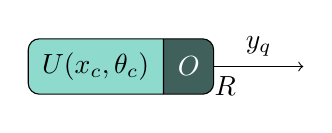
\begin{tikzpicture}
\node[quantum node] (c) at (0,0) {$U(x_c, \theta_c) $ \nodepart{two} $O $};
\draw[->] (c) -- (3.5,0)  node[out label] {$y_{q}$} node[samples label] {$R$};
\end{tikzpicture}
\end{figure}


The variational circuit can be composed of \textbf{layers}
\[ U (\gamma) = \L_{N_L} \cdots \L_{1}\]
which repeat a fixed architecture, which possibly depends on hyperparameters. If there is no layer structure, we set $N_L=1$. A layer $\L_l$, $l=1,...,N_L$, consists of a series of \textbf{gates}
\[\L_l = \G^l_{N_G}(\gamma^l_{N_G}) \cdots \G^l_1(\gamma^l_1). \]
Each gate is parametrised by a set of circuit parameters
$\gamma^i_j$, $i = 1,...,N_L$, $j=1,...,N_G$. The set can be empty if the gate is constant.\\

We propose to use the following \textbf{elementary gate sets} from which the gates $\mathcal{G}$ are taken.

\subsubsection{Qubit architectures}

For qubit architectures we define three parametrized gates,
the elementary rotations around the $x$, $y$ and~$z$ axes:
\begin{eqnarray*}
        R_x(\alpha) &=& \e^{-i\alpha \sigma_x/2} =
        \begin{pmatrix}
          \cos \frac{\alpha}{2} & -i \sin \frac{\alpha}{2}\\
          -i \sin \frac{\alpha}{2} & \cos \frac{\alpha}{2}
        \end{pmatrix}\\
        R_y(\beta) &=& \e^{-i\beta \sigma_y/2} =
        \begin{pmatrix}
          \cos \frac{\beta}{2} & -\sin \frac{\beta}{2}\\
          \sin \frac{\beta}{2} & \cos \frac{\beta}{2}
        \end{pmatrix}\\
        R_z(\gamma) &=& \e^{-i\gamma \sigma_z/2}=
        \begin{pmatrix}
          \e^{-i \frac{\gamma}{2}} & 0\\
          0 & \e^{i \frac{\gamma}{2}}
        \end{pmatrix}\\
\end{eqnarray*}
Any $\SO(3)$ rotation can be expressed using three Euler angles, that is, three rotations around two orthogonal axes. A standard axis choice is~$zyz$. Due to the isomorphism $\SU(2)/\Z_2 \isom \SO(3)$ we obtain a similar \maria{similar to what?} decomposition
for arbitrary single-qubit gates $S$:
\begin{align}
\label{eq:app:euler}
\notag
S &= R_z(\gamma) R_y(\beta) R_z(\alpha)\\
&=
\bpm
e^{-i(\alpha+\gamma)/2} \cos(\beta/2) & -e^{i(\alpha-\gamma)/2} \sin(\beta/2)\\
e^{-i(\alpha-\gamma)/2} \sin(\beta/2) &  e^{i(\alpha+\gamma)/2} \cos(\beta/2)
\epm.
\end{align}

Together with the $\CNOT$ gate this gate set is universal, i.e. any $\SU(2^n)$
gate can be expanded into a finite sequence of $\SU(2)$ and $\CNOT$ gates~\cite{barenco1995}.

\subsubsection{CV architectures}

Most gates in CV quantum computing are naturally parametrised. We consider a universal gate set consisting of a universal Gaussian gate set and a nonlinear gate. The following gates are universal for Gaussian transformations, 
\begin{eqnarray}
  	R(\phi) & =& \exp\left(i \phi \adag \a \right), \\
  	D(\alpha) & =& \exp(r (e^{i\phi} \adag -e^{-i\phi} \a)), \\
  	S(r) & =& \exp \left(\frac{r}{2} \left(e^{-i\phi} \a^2 -e^{i\phi}  (\adag)^2 \right) \right), \\
  	BS(\theta) & =& \exp\left(\eta (e^{i \phi} \adag_1 \a_2 -e^{-i \phi}\a_1 \adag_2) \right).
  \label{Eq:gaussiangates}
\end{eqnarray}
As the nonlinear gate we consider a general transformation
\begin{equation}
	\mathcal{N}(\phi) = \exp(i \phi \; \varphi(\a, \adag))
	\label{Eq:nonlineargate}
\end{equation}
where $\varphi$ is at least of third order in the quadrature operators. 

\subsection{Classical nodes}

A classical node can be any differentiable function $y_c = h(x_c, \theta_c)$ that maps inputs $x_c$ and model parameters $\theta_c$ to real \maria{any need for complex outputs?} output vectors or scalars $y_c$.\\

We depict classical nodes by the following symbol:\\
\begin{figure}[h]
\centering
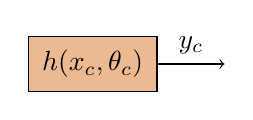
\begin{tikzpicture}
\node[classical node] (c) at (0,0) {$h(x_c, \theta_c) $};
\draw[->] (c) -- (2.5,0)  node[out label] {$y_{c}$};
\end{tikzpicture}
\end{figure}
 


\subsection{Combined nodes}


\begin{figure*}[t]
\begin{flushleft}
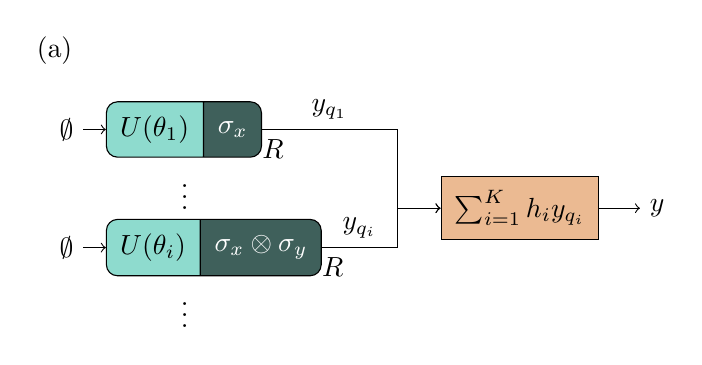
\begin{tikzpicture}
\node[align=left, anchor=west] at (-1,1) {(a)};
\node[input node] (i1) at (-0.5,0) {$\emptyset$};
\node[input node] (iK) at (-0.5,-1.5) {$\emptyset$};
\node[quantum node] (q1) at (0,0) {$U(\theta_1) $ \nodepart{two} $\sigma_x$};
\node[]  at (1,-0.75) {$\vdots $};
\node[quantum node] (qK) at (0,-1.5) {$U(\theta_i)$ \nodepart{two} $\sigma_x \otimes \sigma_y$};
\node[]  at (1,-2.25) {$\vdots $};
\node[classical node] (c) at (4.25,-1) {$\sum_{i=1}^K h_i y_{q_i} $};
\node[output node] (o) at (7,-1) {$y$};
\draw[->] (i1) -- (q1);
\draw[->] (iK) -- (qK) ;
\draw[] (q1.east) -- (3.7,0)  node[out label] {$y_{q_1}$} node[samples label] {$R$};
\draw[->] (3.7,0) -- (3.7,-1)-- (c);
\draw[] (qK.east) -- (3.7,-1.5) node[out label] {$y_{q_i}$} node[samples label] {$R$};
\draw[->] (3.7,-1.5) -- (3.7,-1)-- (c);
\draw[->] (c) -- (o);
%\draw[red] (q1) -| (mid) |- (c.west);
\end{tikzpicture}
 ~~~~~~~~~~~~~~~ 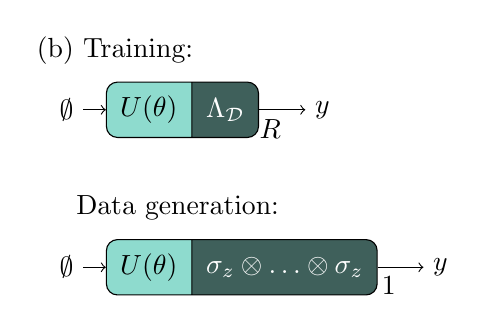
\begin{tikzpicture}
\node[align=left, anchor=west] at (-1,0) {(b) Training:};
\node[input node] (i) at (-0.5,-0.75) {$\emptyset$};
\node[quantum node] (q) at (0,-0.75) {$ U(\theta) $ \nodepart{two} $\Lambda_{\mathcal{D}}$};
\node[output node] (o) at (2.75,-0.75) {$y$};
\draw[->] (i) -- (q);
\draw[->] (q) -- (o) node[samples label] {$R$};
\node[align=left, anchor=west] at (-0.5,-2) {Data generation:};
\node[input node] (i) at (-0.5,-2.75) {$\emptyset$};
\node[quantum node] (q) at (0,-2.75) {$ U(\theta) $ \nodepart{two} $\sigma_z \otimes \hdots \otimes\sigma_z$};
\node[output node] (o) at (4.25,-2.75) {$y$};
\draw[->] (i) -- (q);
\draw[->] (q) -- (o) node[samples label] {$1$};
\end{tikzpicture}\\ \bigbreak

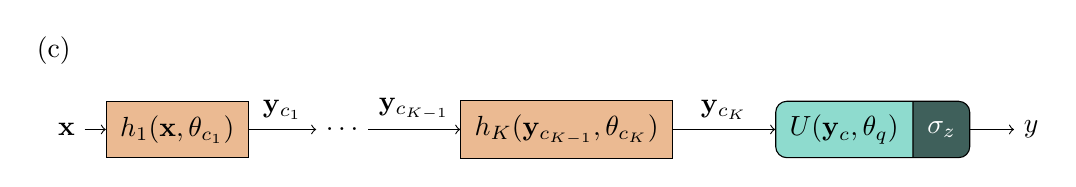
\begin{tikzpicture}
\node[align=left, anchor=west] at (-1,1) {(c)};
\node[input node] (i) at (-0.5,0) {$\bx$};
\node[classical node] (c1) at (0,0) {$h_1(\bx, \theta_{c_1}) $};
\node[] (dots) at (3,0) {$\hdots $};
\node[classical node] (cK) at (4.5,0) {$h_K(\mathbf{y}_{c_{K-1}}, \theta_{c_K}) $};
\node[quantum node] (q) at (8.5,0) {$ U(\mathbf{y}_c, \theta_q) $ \nodepart{two} $\sigma_z$};
\node[output node] (o) at (11.75,0) {$y$};
\draw[->] (i) -- (c1);
\draw[->] (c1) -- (dots) node[out label] {$\mathbf{y}_{c_1}$};
\draw[->] (dots) -- (cK) node[out label] {$\mathbf{y}_{c_{K-1}}$};
\draw[->] (cK) -- (q) node[out label] {$\mathbf{y}_{c_K}$};
\draw[->] (q) -- (o);
\end{tikzpicture}\\ \bigbreak


\end{flushleft}
\caption{Examples of model graphs. Turqois nodes depict quantum nodes, and orange nodes depict classical nodes. (a) Model graph of a variational quantum eigensolver, in which expectation values of local Pauli operators are combined by a classical layer to an expectation value of a global Hamiltonian. (b)  A model, here a generative model) can even have different architectures for training and data generation. While the model is trained maximising the expectation of a quantum operator $\Lambda_{\mathcal{D}}$ that projects onto a `training set subspace' of Hilbert space, it can be used to sample data by performing a single computational basis measurement (i.e., $R=1$). (c) Model graph of a classical neural network with a final quantum layer that computes the scalar output.}
\label{Fig:example_modelgraphs}
\end{figure*}


From the building blocks of classical and quantum nodes, more complicated hybrid structures evolve. Examples of hybrid model graphs are given in Figure \ref{Fig:example_modelgraphs}. Figure \ref{Fig:example_modelgraphs} (a) shows a variational quantum eigensolver, where the model input is an empty set, and the output of the model is the weighed sum of expectation values. Figure \ref{Fig:example_modelgraphs} (b) shows a generative quantum model. Finally, Figure \ref{Fig:example_modelgraphs} (c) shows a classical neural network with one final quantum layer, whose output is the expectation value of a $\sigma_z$ operator applied to a predefined qubit. 



\subsubsection{Cost function}
The cost function has a different structure for different tasks of the learning or optimization task. We distinguish three tasks (see Fig. \ref{Fig:tasks}).\\


\begin{figure}[t]
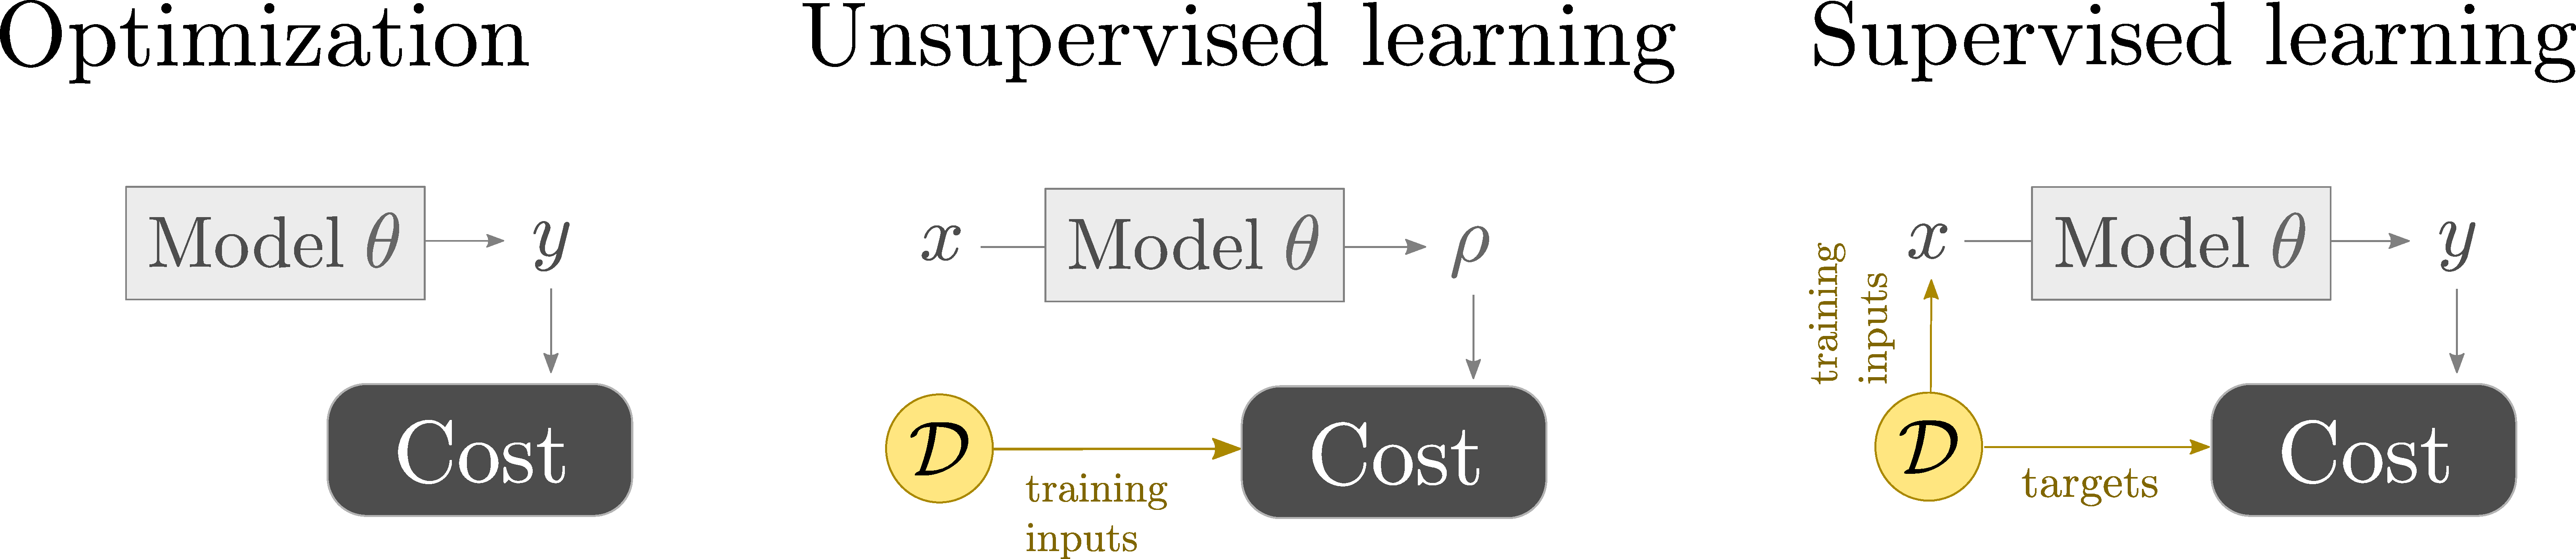
\includegraphics[scale=0.08]{tasks.pdf}
\caption{Three tasks for OpenQML and the ob}
\label{Fig:tasks}
\end{figure}

It is useful to consider some examples
\paragraph{Expectation cost for a variational eigensolver}

The cost function of a variational eigensolver is a weighed sum of expectation values,
\[ C(\theta) = \sum_i h_i E_i(\theta). \]
Usually, these are expectations of Pauli operators, and their sum is the energy expectation,
\[\langle H \rangle = \sum\limits_{i, \alpha} h^i_{\alpha} \langle\sigma^i_{\alpha}\rangle + \sum\limits_{\substack{i,j\\ \alpha, \beta}} h^{ij}_{\alpha, \beta} \langle \sigma^i_{\alpha}\sigma^j_{\beta}\rangle + \hdots,\]
where $i,j$ denote the qubits that the Paulis act on, and
$\alpha, \beta = x,y,z$ sum over all different combinations of Pauli operators.

\paragraph{Cost for a generative model}
If the goal is to increase the likelihood of measuring a basis state
$\ket{x}$ that represents an input in the data set
$\mathcal{D} = \{x\}$, the expectations we are interested in are
\be
E_x(\theta) =  \tr\{\rho(\theta) \ketbra{x}{x}  \},
\ee
and we can use maximum likelihood to define
\[C(\theta, \mathcal{D}) = \sum_{x \in \mathcal{D}}\log E_x(\theta) .\]
Note that in this unsupervised learning task the data enters the cost function directly, and the circuit is data-independent.



\paragraph{Square loss cost for supervised learning}
If we interpret the expectation $E_x(\theta) = \tr \{ \rho(\theta, x)
\; \sigma_z \}$ of the computational basis state of a designated qubit
for an input $x$ as the prediction of a quantum classifier, the square
loss cost function reads
\[ C(\theta, \mathcal{D}) = \sum_{(x,y) \in \mathcal{D}} |E_x(\theta)-y|^2. \]

\color{black}


\section{Gradient computation}

In this section we explore issues related to computing gradients of models $f(x, \theta)$ consisting of quantum and classical nodes with regards to a specific model parameter $\mu \in \theta$.\\

\subsection{Chain rule over nodes}

Assume the model $f$ maps to a scalar output and is a chain of (quantum or classical nodes) $f_1,...,f_T$,
\[ f(x, \theta) = f_T \circ f_{T-1} \circ ... \circ f_1 \in \mathbb{R}.\]
The nodes each take a subset of the parameters $\theta_1,...,\theta_T$. For now we assume that the subsets are disjunct, so that there is no parameter tie. We can formally derive a `backpropagation' mechanism for the model.\\

Let us look at 1-d chains of nodes. The chain rule prescribes that the gradient with respect to a parameter $\mu \in \theta_1$ in the last node is given by
\[ \partial_{\mu} f(x, \theta) =  f_T' \circ f_{T-1} \circ ... \circ f_1, \]
which expresses that $f_T$ is derived for its argument, which consists of the following functions. 
while for general $\mu \in \theta_t$, 
\[ \partial_{\mu \in \theta_t} f(x, \theta) = \prod_{i=1}^t ( f'_i \circ ... \circ f_1 ). \]
(Where obviously $( f'_1 \circ ... \circ f_1 ) = f'_1$ \maria{Is there an iterative symbol for chaining?}).





\subsection{One-parameter subgroups}

A one-parameter subgroup of the topological group~$G$ is defined by a continuous group homomorphism
\be
\phi: \R \to G,
\ee
where $\R$ is a group with respect to addition.
The homomorphism property means that
\be
\phi(a)\phi(b) = \phi(a+b) \quad \forall a,b \in \R,
\ee
which immediately yields
$\phi(0) = e$ and $\phi(-a) = \phi(a)^{-1}$,
where $e$~is the identity element of~$G$.
$\Imag \phi$ is always a subgroup of~$G$.

The kernel of the homomorphism is defined as
\be
\Ker \phi = \{a \in \R | \phi(a) = e\}.
\ee

\begin{theorem}
  \label{th:1psg}
One-parameter subgroups are either isomorphic to~$\R$, or their parametrization~$\phi$ is periodic.

\begin{proof}
$\phi$ is an injection iff $\Ker \phi = \{0\}$ (trivial kernel).
In this case the subgroup $\phi(\R) < G$ is isomorphic to~$\R$.
Let us next assume that the kernel is nontrivial, i.e. for some $p \neq 0$ we have
$\phi(p) = e$.
% p \in \Ker \phi \implies n*p \in \Ker \phi
This is equivalent to
\be
\phi(a+p) = \phi(a)\phi(p) = \phi(a) \quad \forall a \in \R,
\ee
and the map~$\phi$ is thus periodic. Let us use $\tilde{p}>0$
to denote the period, i.e.
$\tilde{p} = \min \{|p| \neq 0 | p \in \Ker \phi\}$.
Now the kernel is seen to be $\Ker \phi = \{n \tilde{p} | n \in Z\}$.
\end{proof}
\end{theorem}

\subsection{Finite-dimensional Hilbert spaces}

Assume we are given a traceless hermitian $n \times n$ generator~$G$, with the eigendecomposition
\be
G = V \diag(\lambda_1, \ldots, \lambda_n) V^\dagger.
\ee
The tracelessness yields $\sum_k \lambda_k = 0$.
$G$~generates a one-parameter subgroup of the unitary group~$SU(n)$
with the homomorphism/parametrization
\be
U(\theta) = \exp(-iG\theta)
= V \diag(e^{-i\lambda_1 \theta}, \ldots, e^{-i\lambda_n \theta}) V^\dagger,
\ee
where $\theta \in \R$. Using Th.~\ref{th:1psg} we find that
\begin{align}
  & U(\theta) \: \text{is periodic with period} \: \tilde{\theta} > 0\\
  \iff \: & \Ker U = \{n \tilde{\theta} | n \in Z\}\\
  \iff \: & \lambda_k \tilde{\theta} = n_k 2 \pi \quad \forall k, \: \text{where} \: n_k \in \Z\\
  \iff \: & \frac{\lambda_i}{\lambda_j} = \frac{n_i}{n_j} \quad \forall i,j
  \: \text{for all nonzero eigenvalues.}
\end{align}

Let us extend the definition of least common multiple to real numbers:
\be
\lcm(a_1, a_2, \ldots) := \min \{q | \forall i \exists n_i \in \Z: a_i n_i = q>0\}.
\ee
Such a number exists iff $a_i$ are rational multiples of each other.
Now
\be
\tilde{\theta} = 2\pi \: \lcm \{\lambda^{-1} \:|\: \lambda \in \spec(G) \setminus \{0\}\}.
\ee



Qubits:
$G$~has only two eigenvalues, and the tracelessness guarantees that $\lambda_2 = -\lambda_1$.
Thus $U(\theta)$ is always periodic with $\tilde{\theta} = 2\pi/|\lambda_1|$.

Qudits:
Now almost all generators~$G$ have eigenvalues that are not rational multiples of each other.
These~$G$ generate a one-parameter subgroup of $U(d)$ isomorphic to~$\R$.
However, some generators~$G$ always generate a periodic subgroup.


\subsection{Gradient trick}

Let us assume $G^2 = r^2\I$.
This is equivalent to $\lambda_i = \pm r$.
Now we may write the Taylor series for the exponential
and split it into a cosine and a sine series:
\begin{align*}
U(\theta) &= \exp(-iG\theta) = \sum_{k=0}^\infty \frac{(-i\theta)^k G^k}{k!}\\
&=
\sum_{k=0}^\infty \frac{(-i\theta)^{2k} G^{2k}}{(2k)!}
+\sum_{k=0}^\infty \frac{(-i\theta)^{2k+1} G^{2k+1}}{(2k+1)!}\\
&=
\I \sum_{k=0}^\infty \frac{(-1)^{k} (\theta r)^{2k}}{(2k)!}
-i G/r \sum_{k=0}^\infty \frac{(-1)^{k} (\theta r)^{2k+1}}{(2k+1)!}\\
&=
\I \cos(r \theta)
-i G/r \sin(r \theta).
\end{align*}
Let us then define the unitary
\be
W := U(\pi/(4r)) = \frac{1}{\sqrt{2}}(\I -ir^{-1}G).
\ee
This yields
\begin{align}
  \notag
\Ad_W \rho
&= W \rho W^\dagger
= \frac{1}{2}\left((\I-ir^{-1}G)\rho(\I+ir^{-1}G)\right)\\
&= \frac{1}{2}\left(\rho -ir^{-1}\ad_G \rho +r^{-2}\Ad_G \rho\right)
\end{align}
and thus we obtain the convenient formula
\be
r(\Ad_W-\Ad_{W^\dagger}) = -i\ad_G.
\ee


Qubits:
This trick works for arbitrary single-qubit gates, generated by a linear combination of Pauli matrices
$G = \vec{a} \cdot \vec{\sigma}/2$
where $|\vec{a}|=1$.
We obtain $G^2 = \frac{1}{4} \I$, and thus $r=1/2$.

Qudits (including the multi-qubit case):
We may use the trick for gates generated by $G$ whose
eigenvalues fulfill $\lambda_i = \pm r$.

\section{Optimization}

OpenQML deals with the optimization of the variational circuit with
regards to the cost. We always minimize the cost. Our core method is
(stochastic) gradient descent.

\subsection{Gradient descent step}
In every \textbf{step} of the optimization algorithm, the parameters are updated according to the following simple loop\\

\begin{algorithmic}[1]
\Procedure{Gradient descent step}{}
\State [sample a batch $\mathcal{D}$ from the training data]
\For {$\mu \in \theta $}
\State $\mu^{(t+1)} = \mu^{(t)} - \eta^{(t)} \partial_{\mu} C(\theta[, \mathcal{D}]) + S$
\EndFor
\EndProcedure
\end{algorithmic}

The learning rate $\eta^{(t)}$ can be adapted in each step, either
depending on the gradient or on the step number. $S$ is a potential
additional term that can add a momentum to the update. The gradient
$\partial_{\mu} C(\theta[, \mathcal{D}])$ has to be evaluated by
automatic differentiation of the cost function, which is computed
hybridly by the quantum device or simulator and a classical
computer. We therefore need to define a hybrid automatic
differentiation scheme.

\subsection{Computing the gradient}
For the cost of Eq. (\ref{eq:cost}) and neglecting the dependency on inputs $x$ for now, we have
\[\partial_{\mu} C(\theta[, \mathcal{D}]) = \sum_i \frac{d g(\{E_i(\theta)\})}{d E_i(\theta)} \partial_{\mu} E_i(\theta). \]
The first gradient $\frac{d g(\{E_i(\theta)\})}{d E_i(\theta)}$ is the
derivative of the classically computed part of the cost. We evaluate
it using standard computational tools for automatic
differentiation. The second gradient $\partial_{\mu} E_i(\theta)$ is
the derivative of the part that is computed by the quantum device. We
need something like ``quantum automatic differentiation'' to compute
these gradients.

Formally, we have
\begin{eqnarray*}
        \partial_{\mu} E_i(\theta) &=& \partial_{\mu} \tr \{\rho(\theta) \; \hat{O}_i\} \\
        &=& \tr \{ (\partial_{\mu}  \rho(\theta)) \; \hat{O}_i\}, \\
\end{eqnarray*}
and with $\rho(\theta) = U(\theta)\rho_0U^{\dagger}(\theta)$ and the product rule of differentiation, we get
\[\partial_{\mu}  \rho(\theta) = \left(\partial_{\mu}   U(\theta)\right) \rho_0U^{\dagger}(\theta) +   U(\theta) \rho_0 \left(\partial_{\mu} U^{\dagger}(\theta)\right)   . \]
This expression contains the \textbf{circuit derivative},
$\partial_{\mu}  U(\theta)$. Assume that only the $l$th layer depends
on circuit parameter $\mu$, then
\[
\partial_{\mu}  U(\theta) =  \mathcal{L}_1^{\dagger} \cdots (\partial_{\mu} \mathcal{L}_l^{\dagger})\cdots \mathcal{L}_D^{\dagger}.
\]
We call the expression $\partial_{\mu} \mathcal{L}_d^{\dagger}$  the
\textbf{layer derivatives}. The layer is decomposed into different
gates from our universal gate set. Let $\mu$ be the parameter of the
$r$th gate $\G_r(\mu)$ (where $\G$ can also depend on other
parameters). The derivative of a layer is then the original layer, but
instead of $\G_r$ we use $\partial_{\mu} \G_r(\mu)$. This expression
is in general not a quantum gate, and in particular not necessarily a
member of our elementary gate set. We therefore have to decompose it
into a weighed sum of ``allowed gates'' $A_k(\mu)$,
\begin{equation}
        \partial_{\mu} \G(\mu) = \sum_k a_k A_k(\mu),
    \label{eq:decomposition_derivative}
\end{equation}
with complex coefficients $a_k$. This is always possible, because any
operator can be represented as a sum of unitaries, and if our
elementary gate set is universal for quantum computing, it can
represent any unitary. The derivative circuit hence becomes
\begin{eqnarray}
\partial_{\mu}  U(\theta)  &=& \sum_k a_k U_{A_k}(\theta) \\
&=& \sum_k a_k \G_1^1 \cdots A_k(\mu) \cdots \G_{N_G}^{N_L},
\end{eqnarray}
where $U_{A_k}(\theta)$ is the original circuit but with the gate $\G_r^l(\mu)$ replaced by $A_k(\mu)$. \\



An example is the special case for Equation (\ref{eq:decomposition_derivative}) when $\G(\mu) = \e^{i\mu H}$ for a generator $H$. Then, formally,
\[
\partial_{\mu}\G(\mu) = i H \e^{i\mu H}.
\]
Since $H$ might not be a unitary operator, we have to decompose it into unitaries $H_k$ via $H = \sum_k a_k H_k$, so that
\[
\partial_{\mu}\G(\mu) = \sum_k i \underbrace{H_k \e^{i\mu H}}_{A_k}.
\]

Summarizing the above, we get the formulae
\begin{eqnarray*}
        \partial_{\mu} E_i(\theta) &=& \tr \{ \sum_k \left[ a_k  U_{A_k}(\theta) \rho_0 U^{\dagger}(\theta) + h.c. \right] \; \hat{O}_i\}, \\
        &=& \sum_k \tr \{  \left[ a_k  U_{A_k}(\theta) \rho_0 U^{\dagger}(\theta) + h.c. \right] \; \hat{O}_i\}\\
        &=& \sum_k \tr \{   a_k  U_{A_k}(\theta) \rho_0 U^{\dagger}(\theta) \hat{O}_i + h.c. \}.
\end{eqnarray*}

Altogether, the quantum computer has to evaluate the terms
\[ \tr \{  U_{A_k}(\theta) \rho_0 U^{\dagger}(\theta)  \hat{O} \},\]
and
\[ \tr \{  U(\theta) \rho_0 U_{A_k}^{\dagger}(\theta)  \hat{O} \},\]
from which we can construct the derivative of the expectation classically. For this, we have to prepare a quantum state of the form
\[ \mathcal{A} \rho_0 \mathcal{B}, \]
where $ \mathcal{A}, \mathcal{B}$ are the derivative and the original variational circuit. \\

\maria{Nathan, you mentioned that you know a trick of how we can implement this easily? So far I am very sceptical that this is simple. I only know the following trick:
Decompose $\hat{O}$ into a sum of unitaries $B_s$,
\[\hat{O} = \sum_s b_s B_s,\]
so that we have to implement
\[ \tr \{  U(\theta) \rho_0 U_{A_k}^{\dagger}(\theta)  B_s \}.\]
Define $A=U(\theta)$ and $D=U_{A_k}^{\dagger}(\theta)  B_s$, then prepare
\[ \frac{1}{\sqrt{2}} (\ket{0} \otimes A\rho_0 A^{\dagger} + \ket{1} \otimes D\rho_0 D^{\dagger}),\]
and apply a Hadamard on the ancilla. The probability of measuring the ancilla in $0$ is
\[p(0) = \frac{1}{2} + \frac{1}{2} \tr \{ A\rho_0 A^{\dagger} D\rho_0 D^{\dagger} +D\rho_0 D^{\dagger} A\rho_0 A^{\dagger}  \} \]
For this, the quantum device needs ancilla qubits, and $A_k$ and $B_s$ have to be implemented conditioned on the ancilla. }

%\bibliographystyle{unsrt}
\bibliography{openqml_formalism}


\end{document}
